\section{Methodology and Results}
In this section, I describe the steps that I have taken to reduce the number of features and to cluster the date generated in the previous section.

\subsection{Scaling}
To make sure that all features affect both the PCA and the subsequent clustering in the same way, I apply min-max scaling. This is done by the script \textbf{\emph{rescale\_before\_clustering.py}}. The produced set is referred to as the \emph{rescaled set}.

\subsection{Feature Reduction with PCA}
\subsubsection{PCA Motivation}
The application of a feature reduction technique has various advantages for the problem at hand. It \textbf{a)} enables an easier (two-dimensional) visualization of the clustering results, \textbf{b)} creates hidden features that enable a better interpretation of the clustering results, and \textbf{c)} may improve the results of the clustering as the complexity is reduced with fewer features.

I have chosen PCA as the feature reduction technique. Processing the averaged set by the script \textbf{\emph{apply\_pca.py}} produces the \emph{two principal components} set. 

\subsubsection{PCA Result Discussion}

\paragraph{Number of Principal Components}
I have decided to use tow principal components. This is mainly motivated by the fact that I would like to visualize the clustering results and that this is much easier with two features. However, the two first principal components have a combined explained variance of 0.67, so that we lose some information through the application of PCA. 

\paragraph{Feature Distribution - First Principal Component}
Figure \ref{fig_pc1} illustrates how the first principal component is calculated based on the features from the average set. As can be seen, this component is mainly affected by the features \textbf{Incorrects}, \textbf{Correct First Attempt}, and \textbf{Hints}. A student who had many incorrect attempts, rarely solved the problems with his/her first attempt, and required a lot of hints will have high values in this feature. Overall, I interpret this feature as a hidden measurement on the success that the student had while solving the problems. This feature is well suited for the usage by a tutor because it allows him to judge how often the students get the problems right. Students who rarely end up with the correct answer will have a high value in this feature.

  \begin{figure}
  	\centering
  	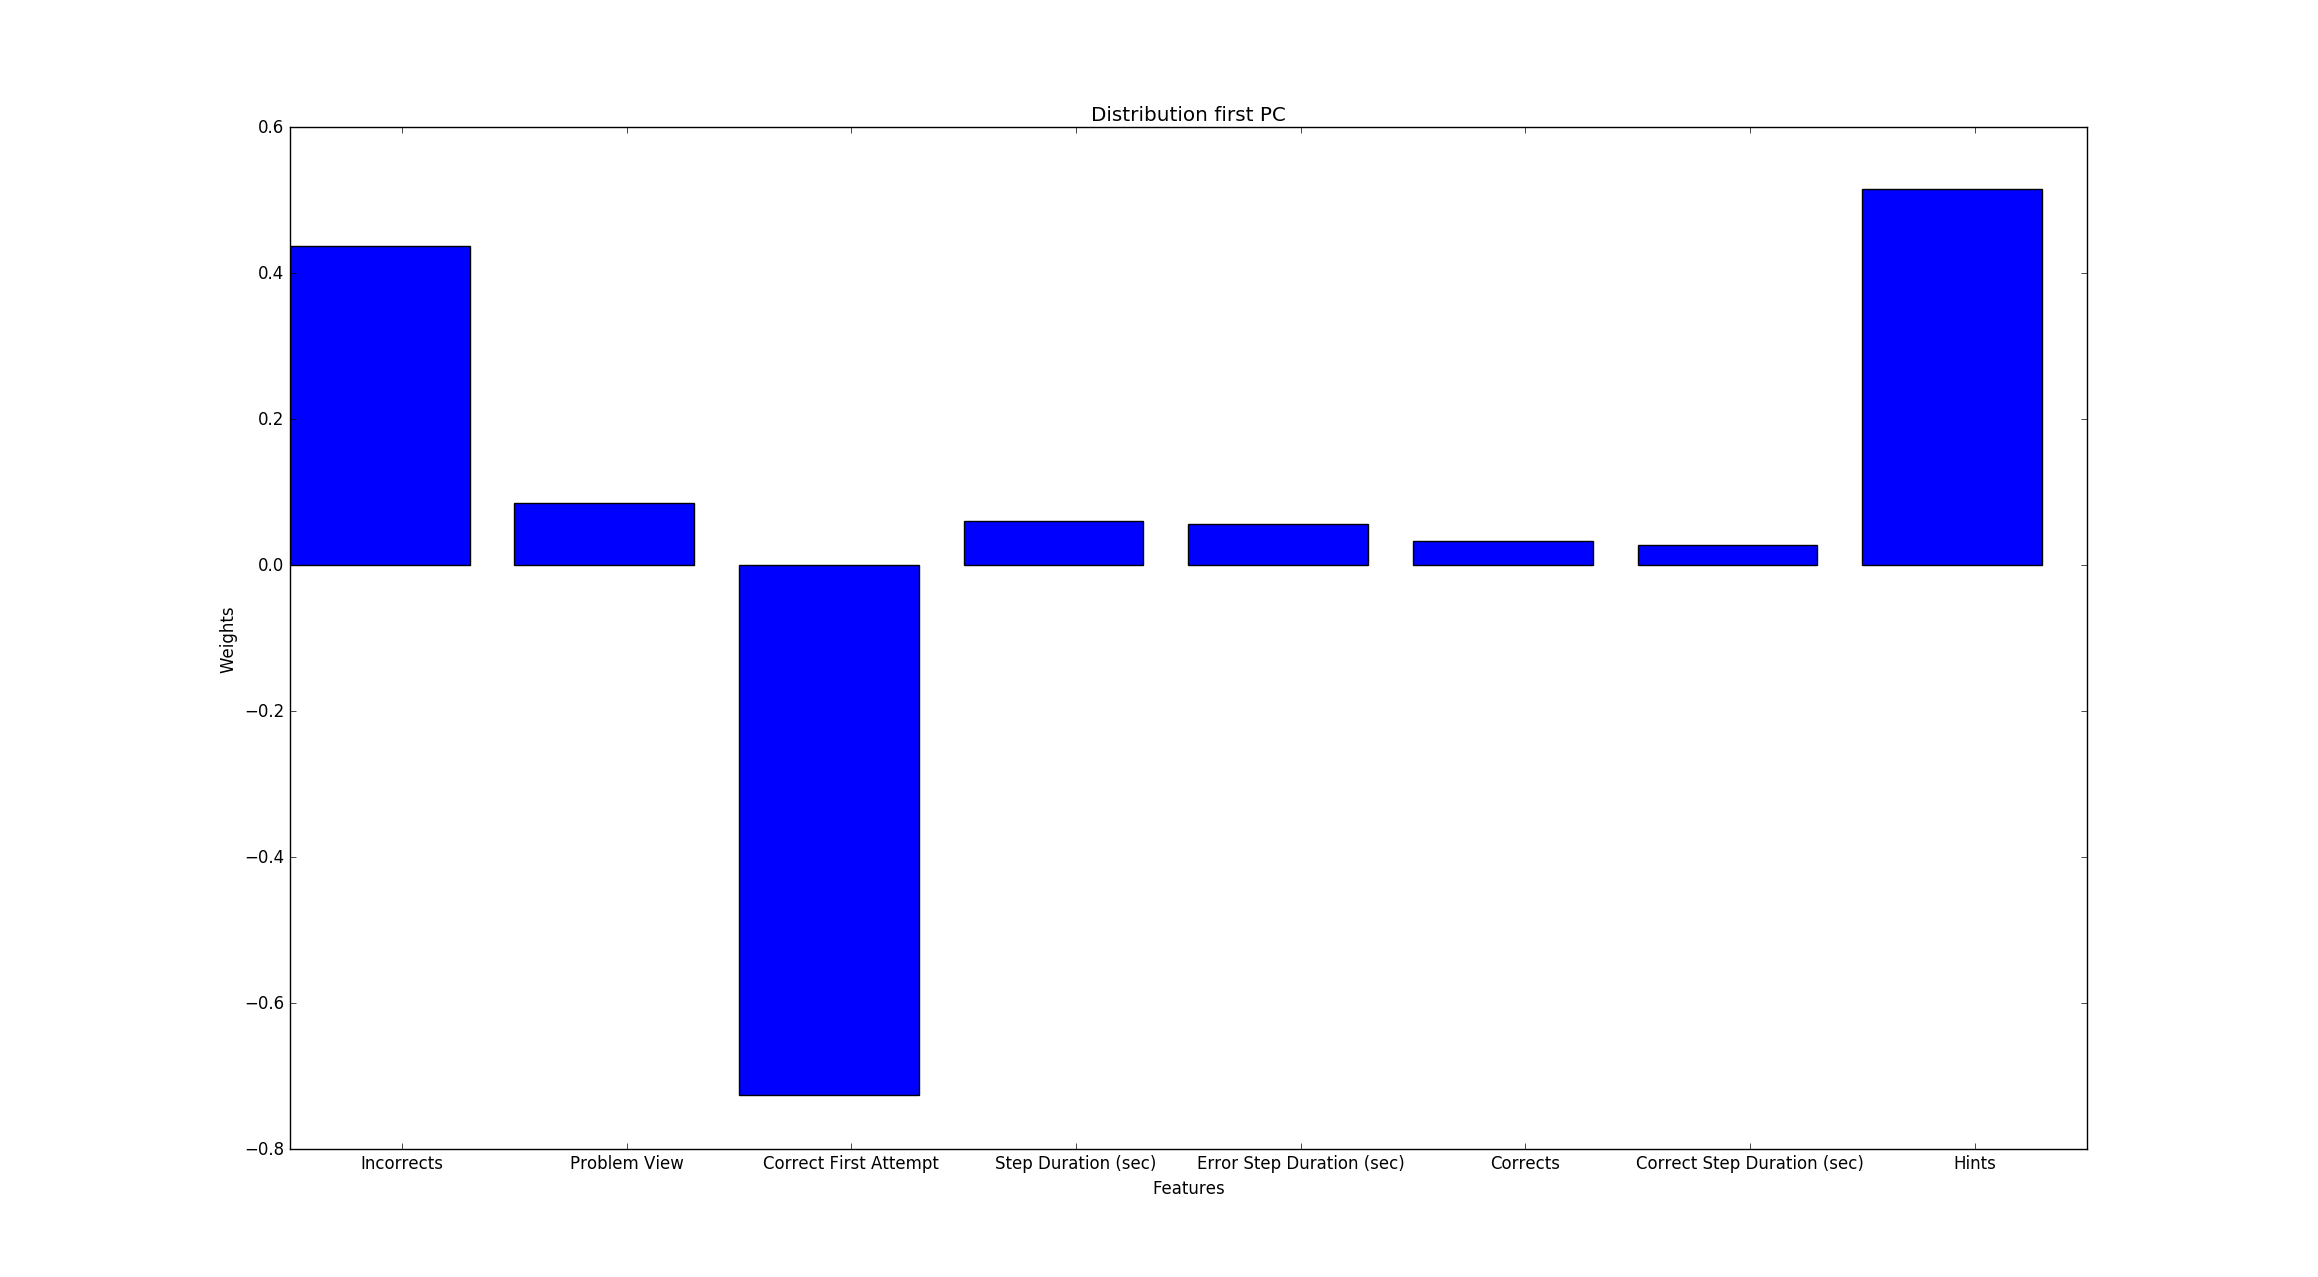
\includegraphics[width=\textwidth]{./img/pc1.png}
  	\caption{The first principal component is mainly affected by the features \textbf{Incorrects}, \textbf{Correct First Attempt}, and \textbf{Hints}. It, consequently, mainly describes whether the student solved the problems correctly and on his/her own.\label{fig_pc1}}
  \end{figure}
  
\paragraph{Feature Distribution - Second Principal Component}
Figure \ref{fig_pc2} illustrates how the second principal component is calculated based on the features from the average set. As can be seen, this component is mainly affected by the features \textbf{Step Duration}, \textbf{Error Step Duration}, and \textbf{Correct Step Duration}. This hidden feature will, consequently be high for a student who needed a long time for the problems. As both the correct and the incorrect step duration are taken into account here, the main focus of this feature is on the time that was needed to provide the solution and not on the question whether the solution was correct. The second principal component is also well suited to be used by a tutor to describe the students, as it allows him/her to describe whether the students are rather fast or rather slow when solving the problem. 

  
    \begin{figure}
    	\centering
    	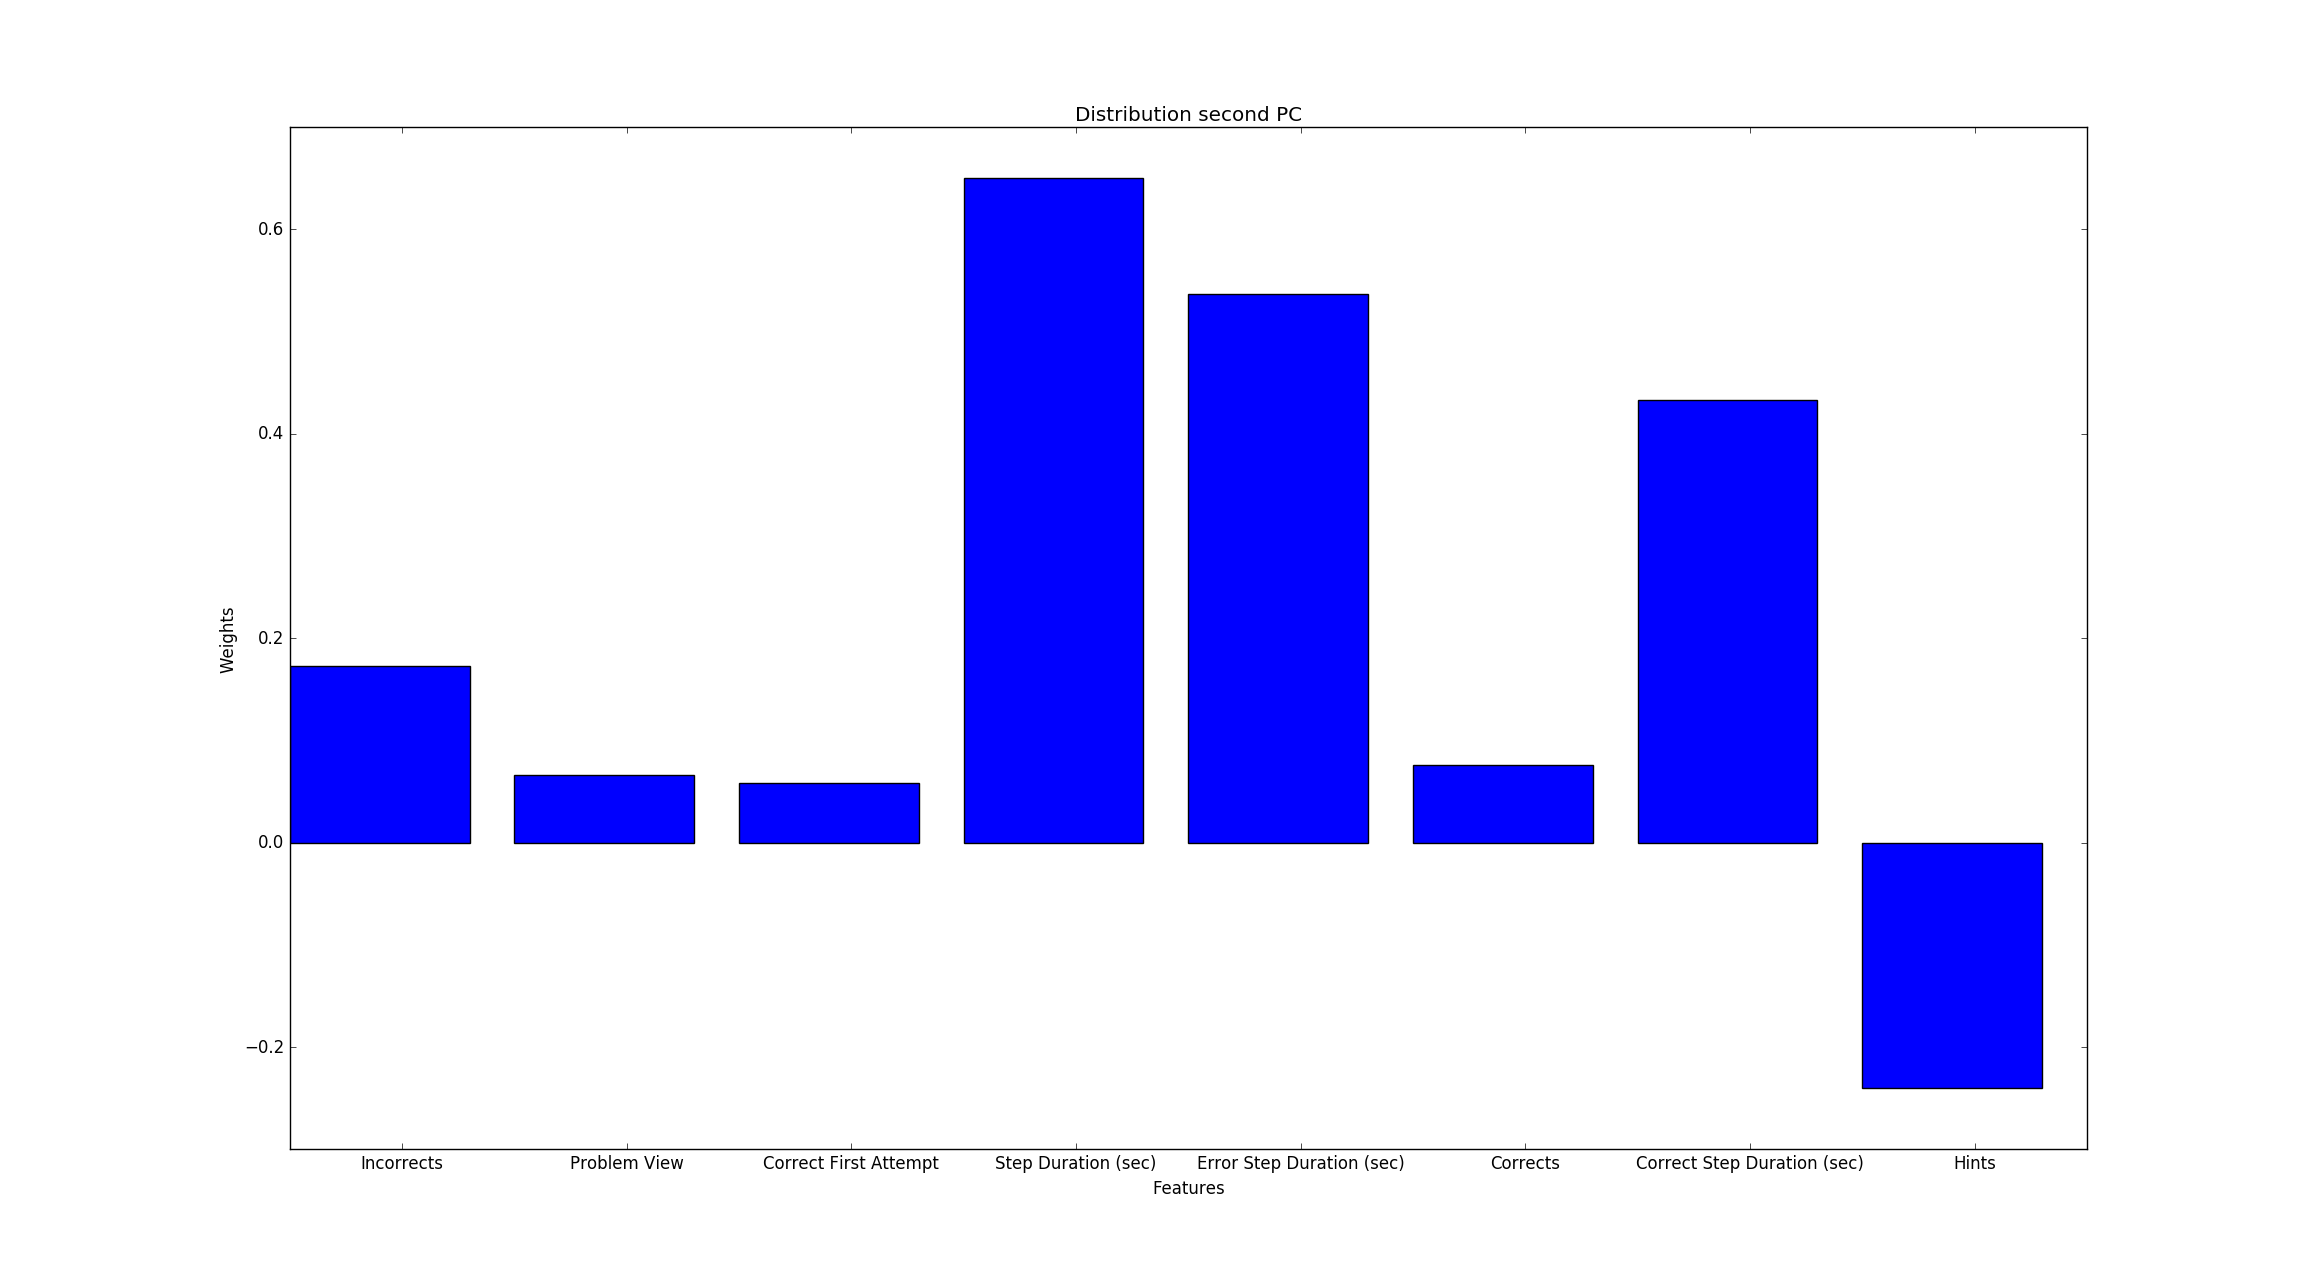
\includegraphics[width=\textwidth]{./img/pc2.png}
    	\caption{The second principal component is mainly affected by the features \textbf{Step Duration}, \textbf{Error Step Duration}, and \textbf{Correct Step Duration}. It, consequently, mainly describes how much time the student spent with the problem.\label{fig_pc2}}
    \end{figure}
    
\subsection{Clustering of the Data}
There are three important decisions that have to be made before actually applying a clustering algorithm. On the one hand, the number of clusters has to be decided. For the problem at hand, the number of clusters describes the number of groups used to describe the students. On the other hand, the algorithm that will be used for the clustering has to be chosen. Finally, a benchmark has to be chosen to evaluate the clustering results.  

\subsubsection{Shape of the Data}
The data obtained from the PCA step is illustrated in Fig.~\ref{fig_data_shape}. Each point represents that data of one student. One noticeable quality of the data is the fact that most of the students can be found near the left lower corner of the plot. This means that most students have rather low values in both principle components, meaning that their solutions were relatively correct and that they solved the problems in a relatively short amount of time.  

\begin{figure}
	\centering
	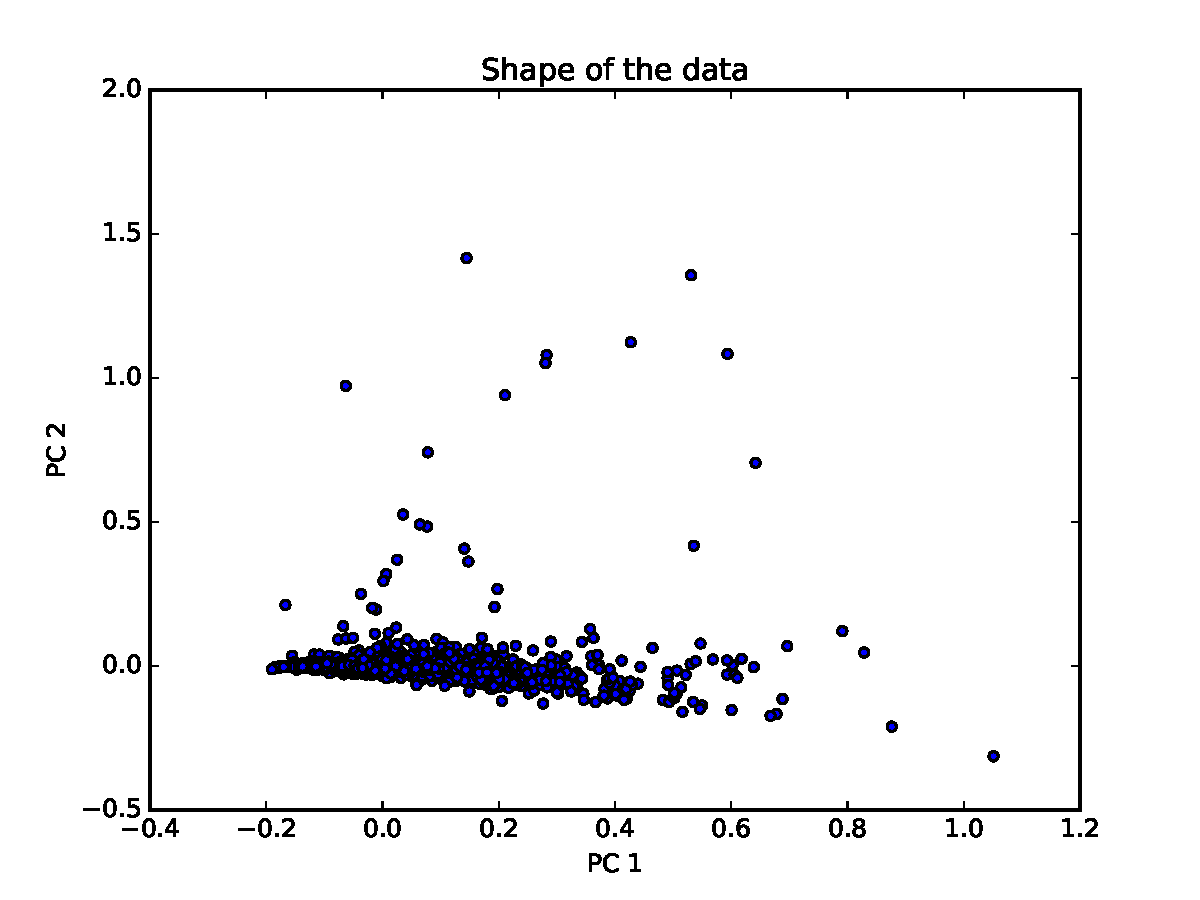
\includegraphics[width=.5\textwidth]{./img/data_shape.pdf}
	\caption{Shape of the data after the PCA step.\label{fig_data_shape}}
\end{figure}

\subsubsection{Choosing the Number of Clusters.}
All the figures introduced in this subsection were created using the script \textbf{\emph{cluster.py}}. I chose the silhouette score to evaluate the clustering when used with cluster numbers ranging from 2 to 5. I used the GMM clustering algorithm for this step. The resulting clusters are plotted in Fig.~\ref{fig_cluster_numbers} while the Fig.~\ref{fig_silhouette} illustrates the the silhouette score for the different cluster numbers. The clustering algorithm never finds more than 3 different groups to distribute the students. In addition, the silhouette score is highest when using two clusters. Using only two groups for the student classification also has a practical advantage, as it will be easier for the tutors to assign a student to one of two instead to one of three groups. 

\begin{figure}[h]
	\centering
	
	\subfloat[2 Clusters]{
		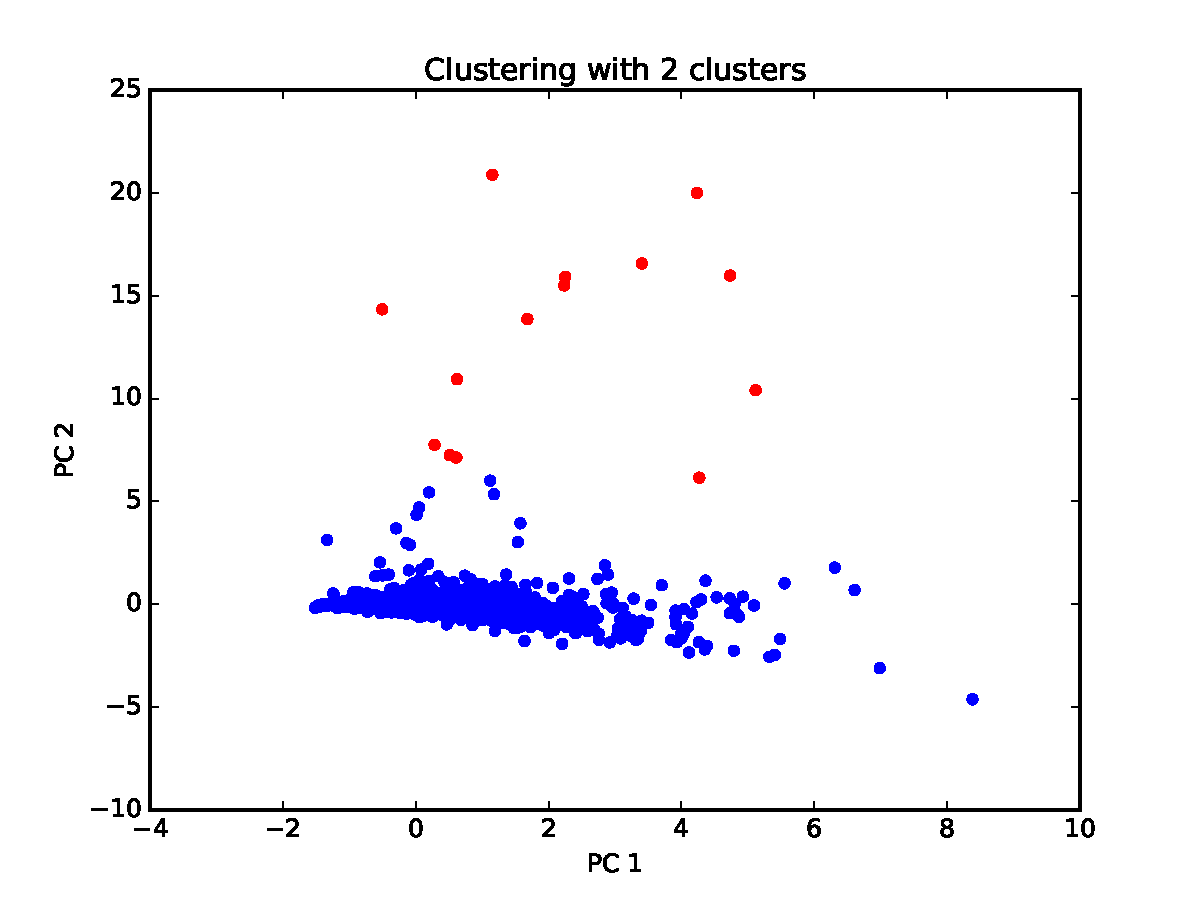
\includegraphics[width=.5\textwidth]{./img/n_clusters_2.pdf}}
	\subfloat[3 Clusters]{
		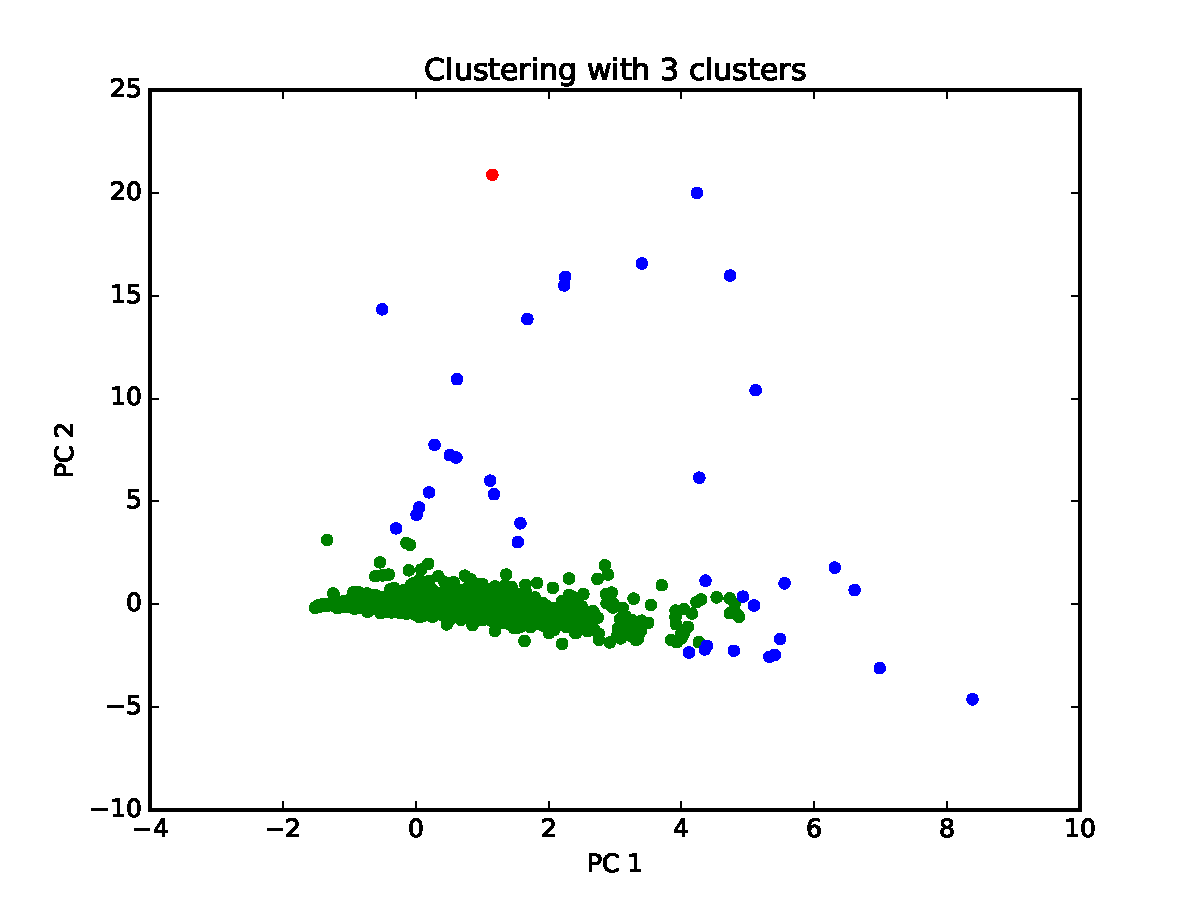
\includegraphics[width=.5\textwidth]{./img/n_clusters_3.pdf}}
	
	
	\subfloat[4 Clusters]{
		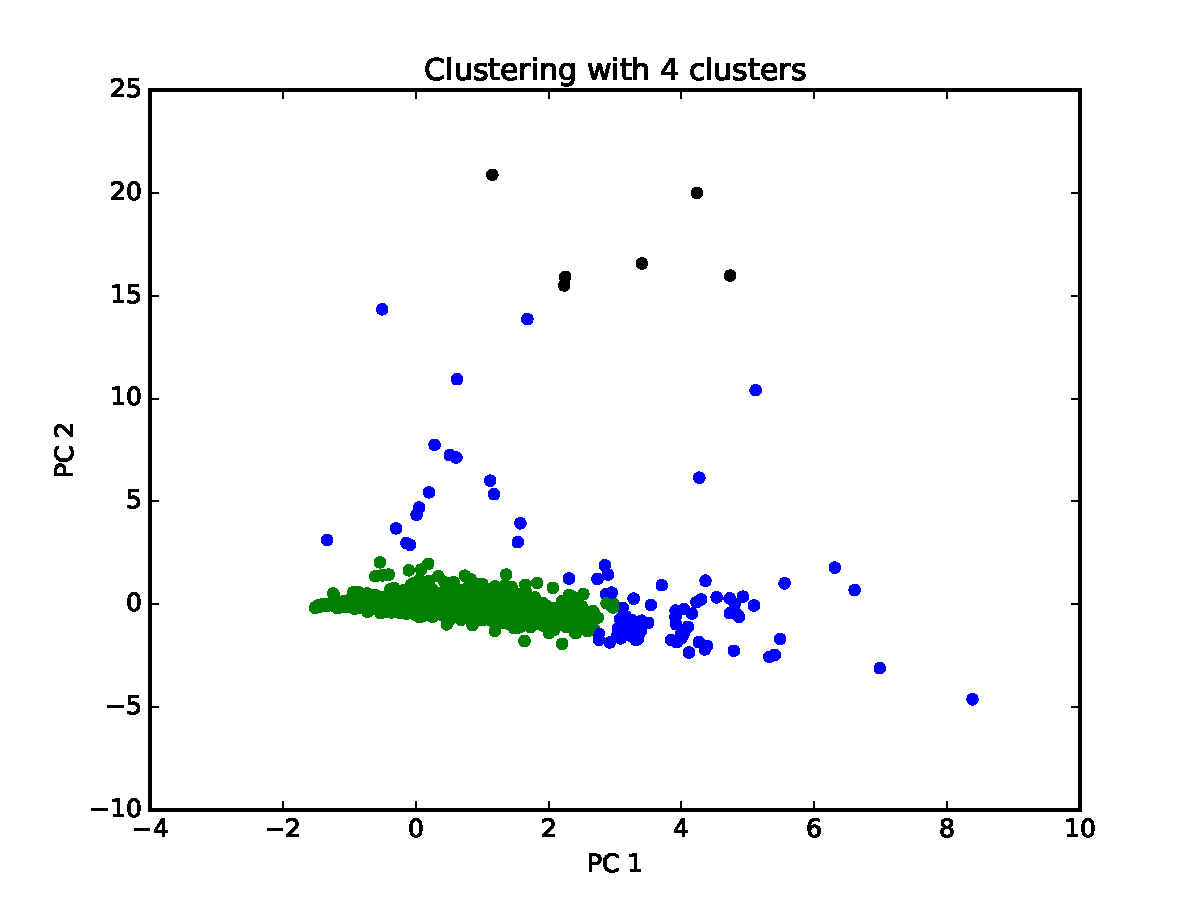
\includegraphics[width=.5\textwidth]{./img/n_clusters_4.pdf}}
	\subfloat[5 Clusters]{
		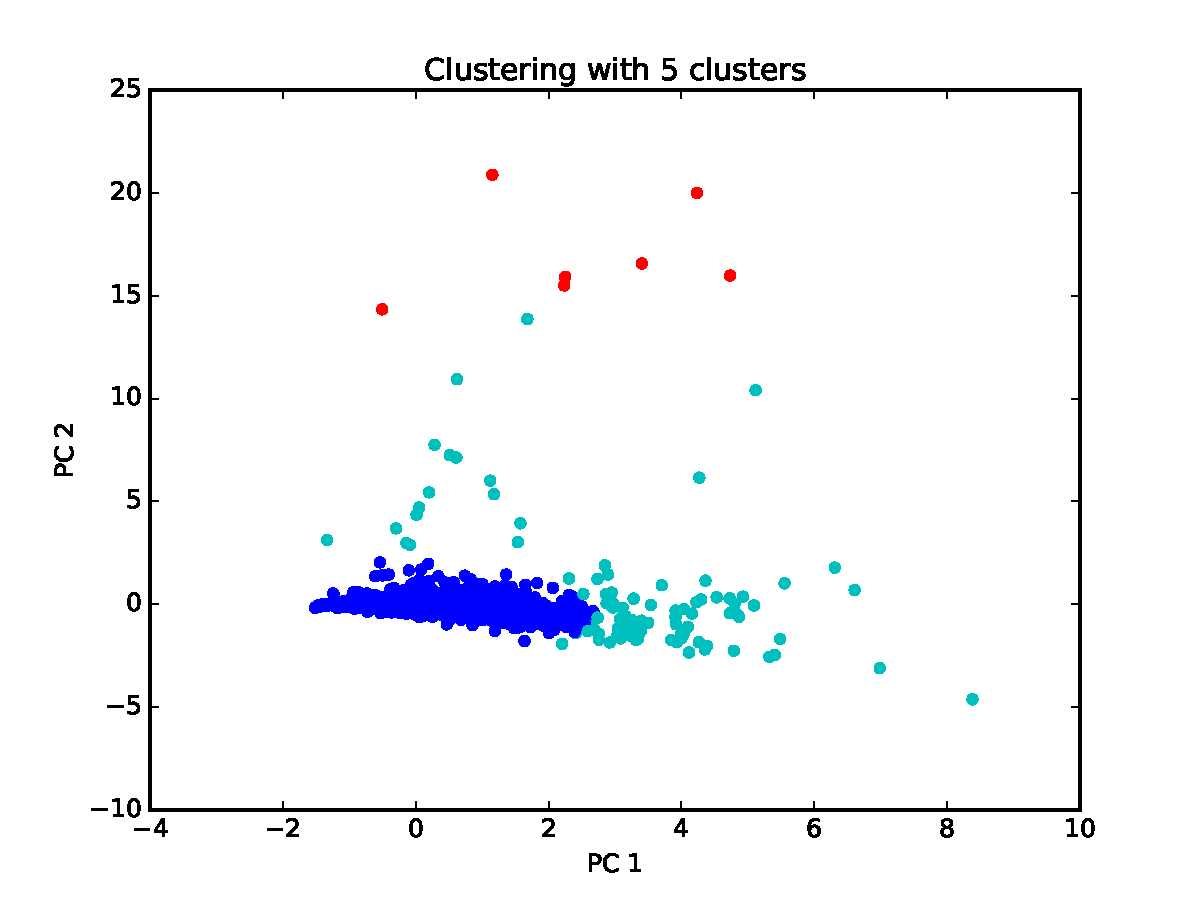
\includegraphics[width=.5\textwidth]{./img/n_clusters_5.pdf}}
	\caption{The results of the clustering for different numbers of clusters.}
	\label{fig_cluster_numbers}		
\end{figure}



    \begin{figure}
    	\centering
    	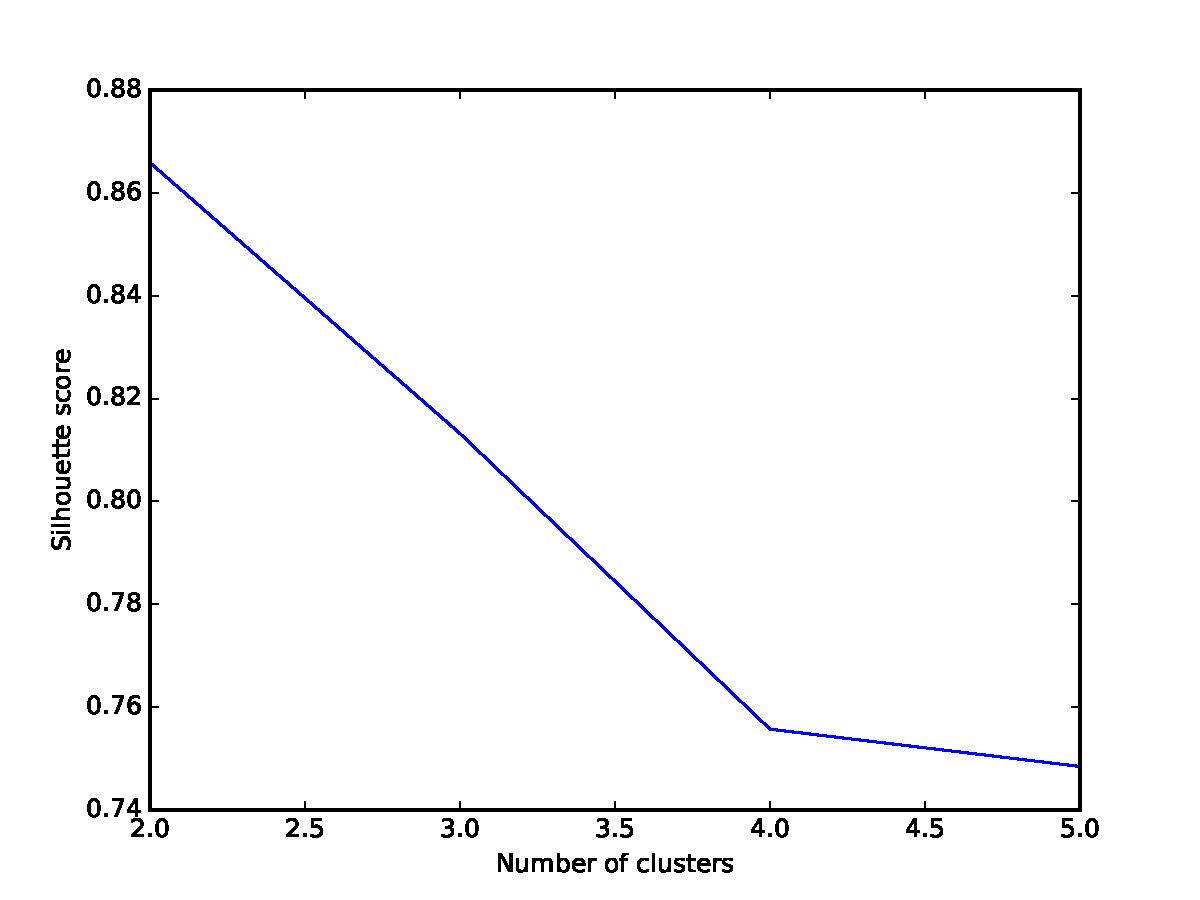
\includegraphics[width=.5\textwidth]{./img/silhouette.pdf}
    	\caption{The silhouette score indicates that the most distinct clustering is obtained with 2 clusters.\label{fig_silhouette}}
    \end{figure}
    
\subsubsection{Choosing and Creating a Benchhmark.}
As described in the capstone proposal, I want to evaluate the clustering by comparing the clustering result with a student clustering that is done solely based on the correctness score of the student. The bench mark is created using the script \textbf{\emph{create\_benchmark.py}}. Fig.~\ref{fig_bench} illustrates the division in groups created as benchmark when using two and five groups. As I have decided to use two clusters, it is sensible to also use the benchmark with 2 groups.


\begin{figure}[h]
	\centering
	\subfloat[2 Groups (split in the middle)]{
		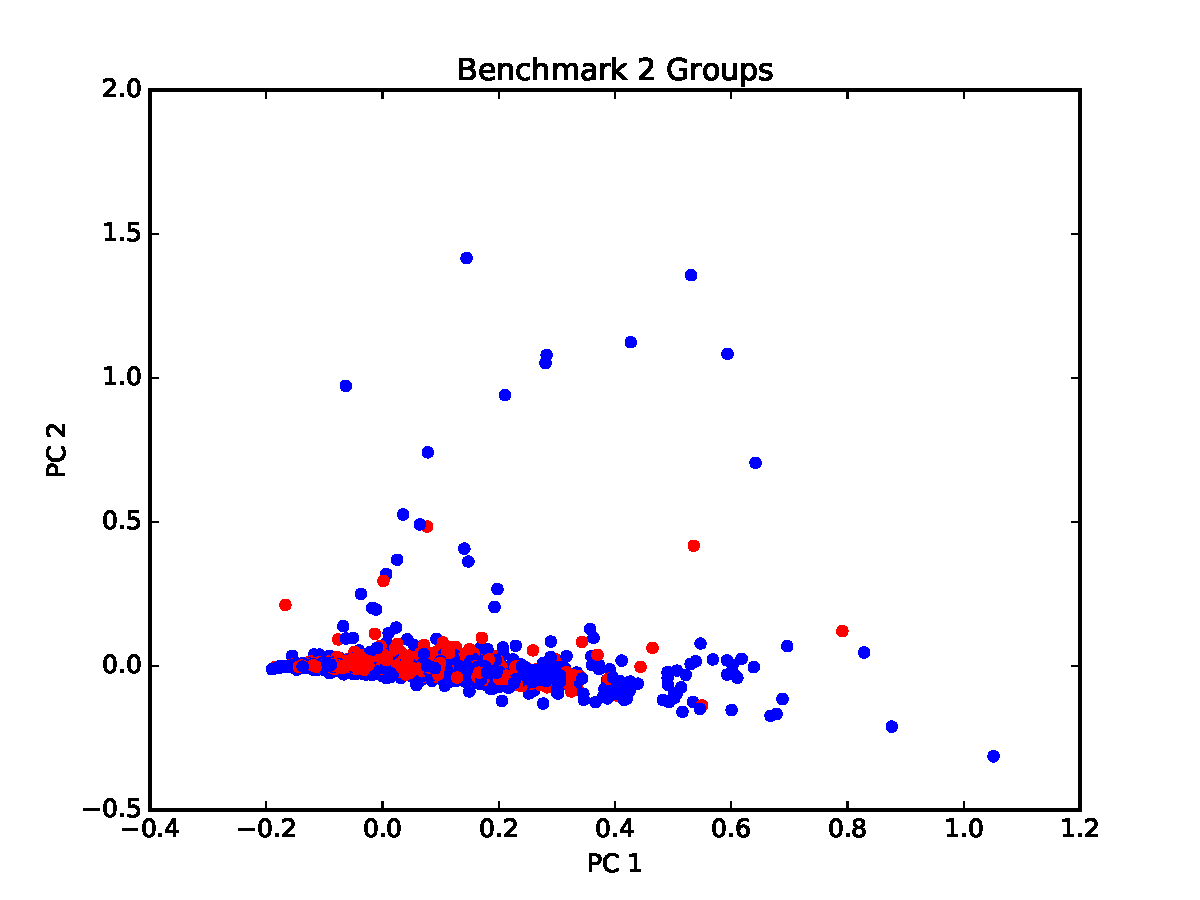
\includegraphics[width=.5\textwidth]{./img/bench_2.pdf}}
	\subfloat[5 Groups]{
		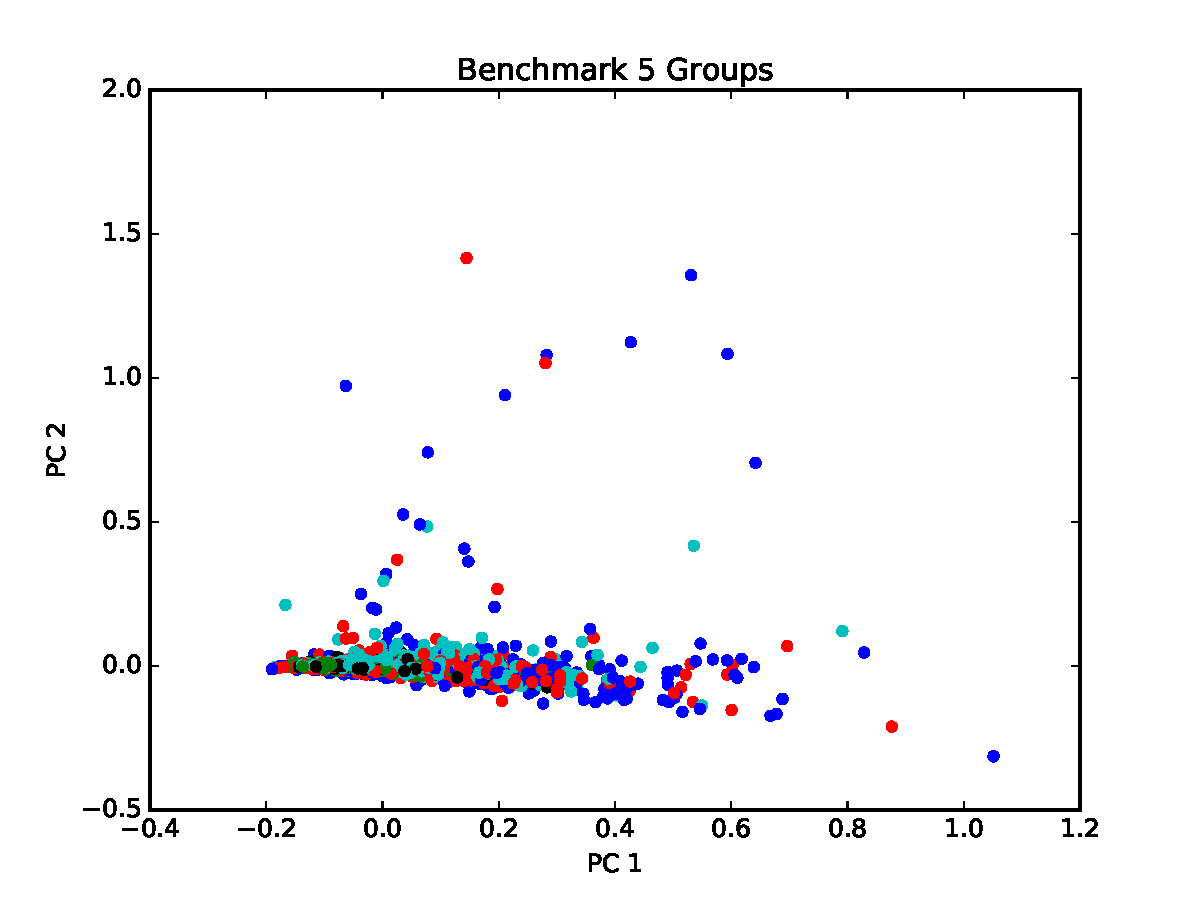
\includegraphics[width=.5\textwidth]{./img/bench_5.pdf}}
	\caption{Distribution of the benchmark groups.\label{fig_bench}}		
\end{figure}


\subsubsection{Choosing the Clustering Algorithm.}

Having decided that I want to cluster the students into 2 groups, the last step is to pick the clustering algorithm that is to be used. Fig.~ illustrates the results of the clustering when using different algorithms. These plots are created using the script \textbf{\emph{comparison.py}}.

\begin{figure}[h]
	\centering
	\subfloat[Agglomerative Clustering (23 \%)]{
		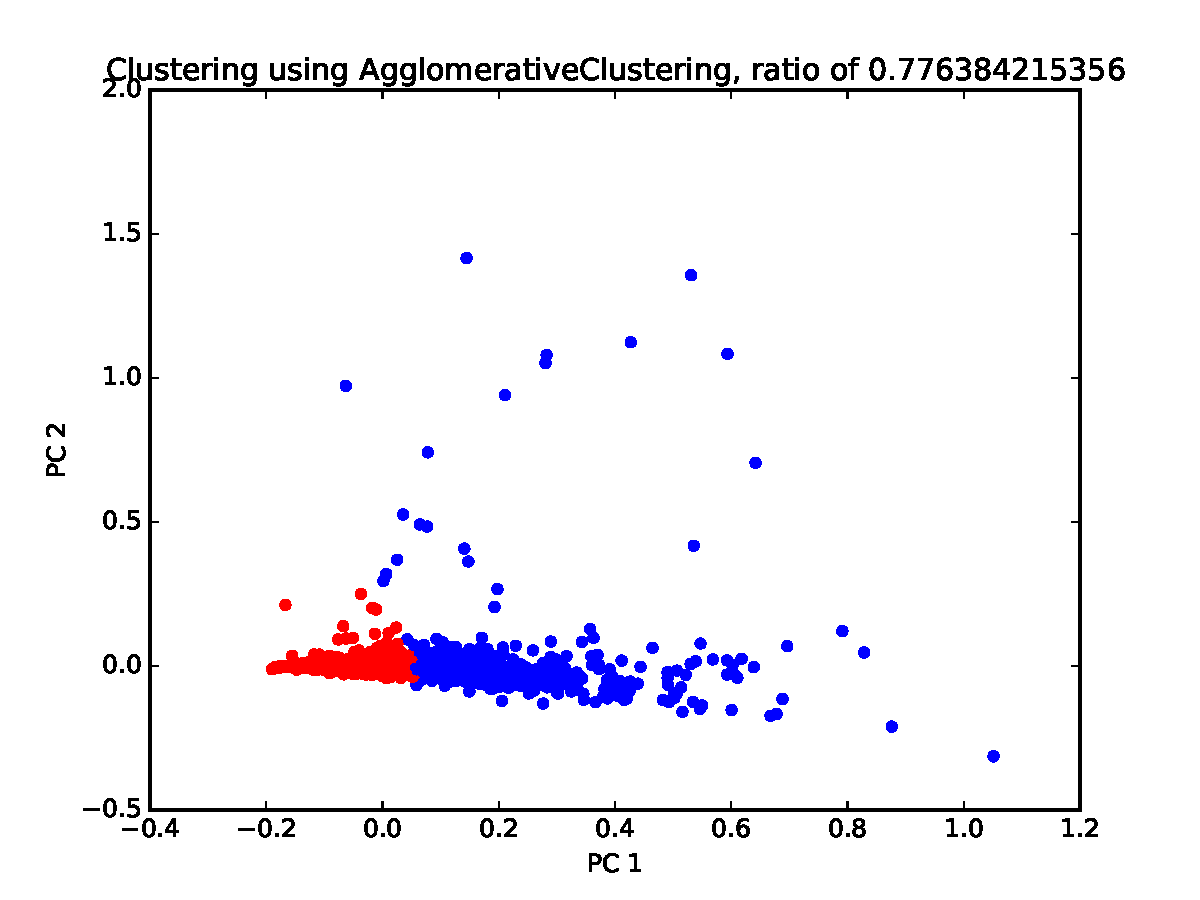
\includegraphics[width=.32\textwidth]{./img/comp_Agglomerative_23.pdf}}
	\subfloat[Birch (0.3 \%)]{
		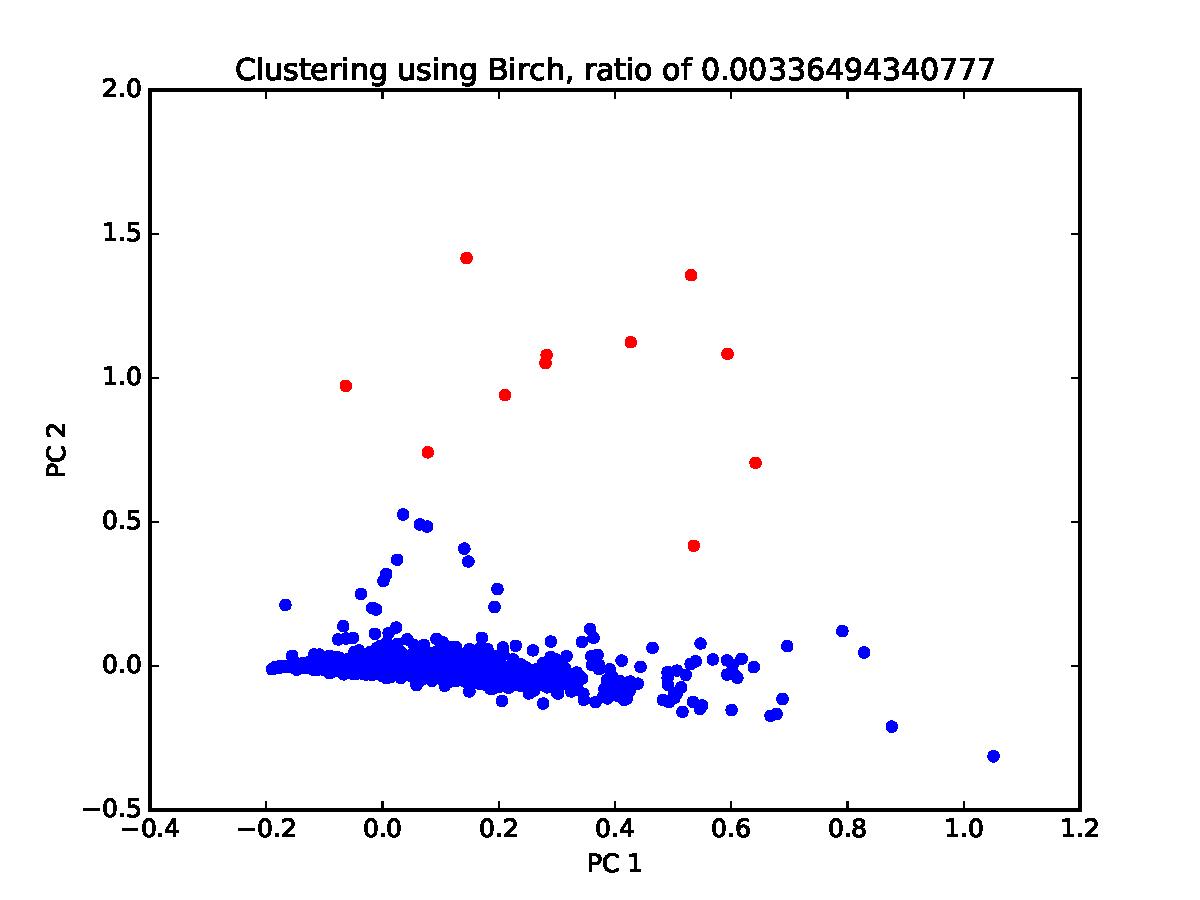
\includegraphics[width=.32\textwidth]{./img/comp_Birch_003.pdf}}
	\subfloat[DBSCAN (0.0 \%)]{
		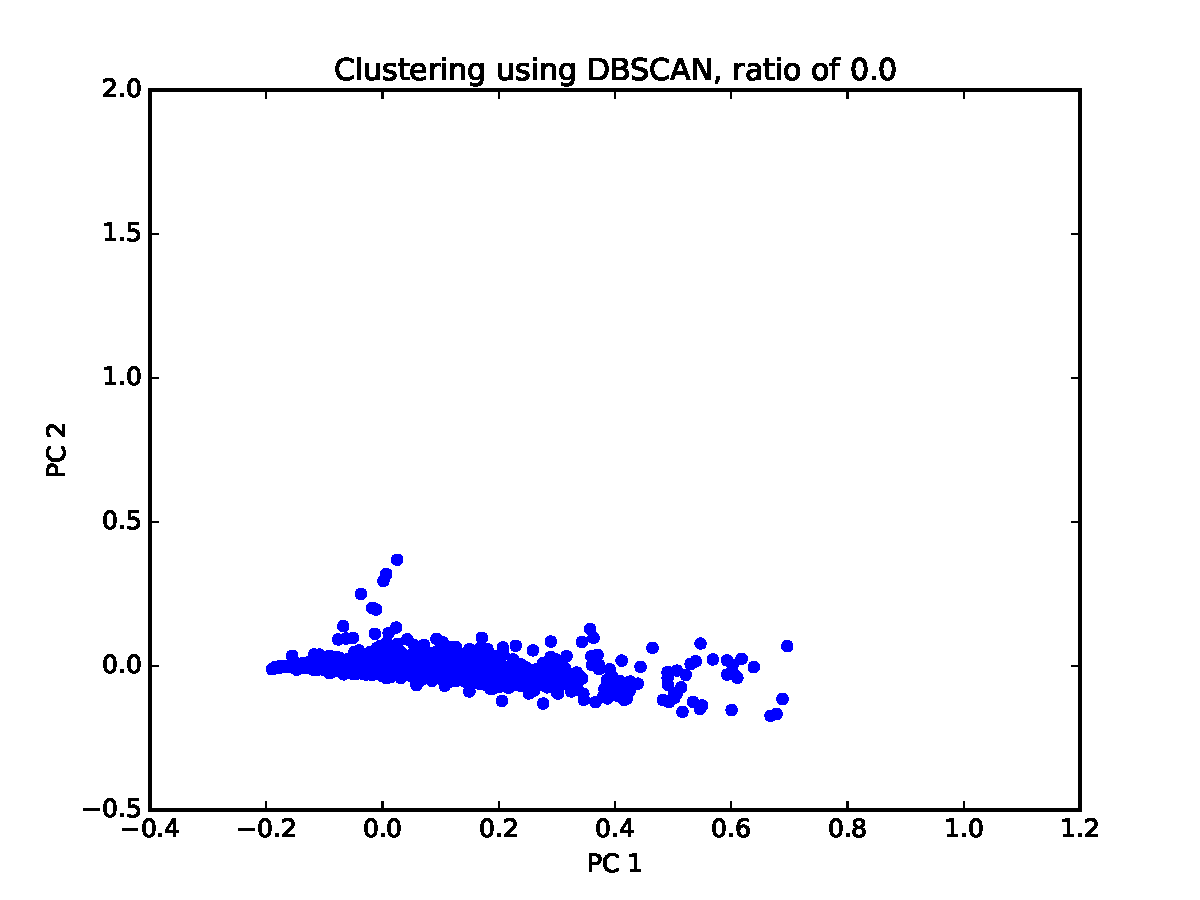
\includegraphics[width=.32\textwidth]{./img/comp_DBSCAN.pdf}}
	
	\subfloat[GMM (4 \%)]{
		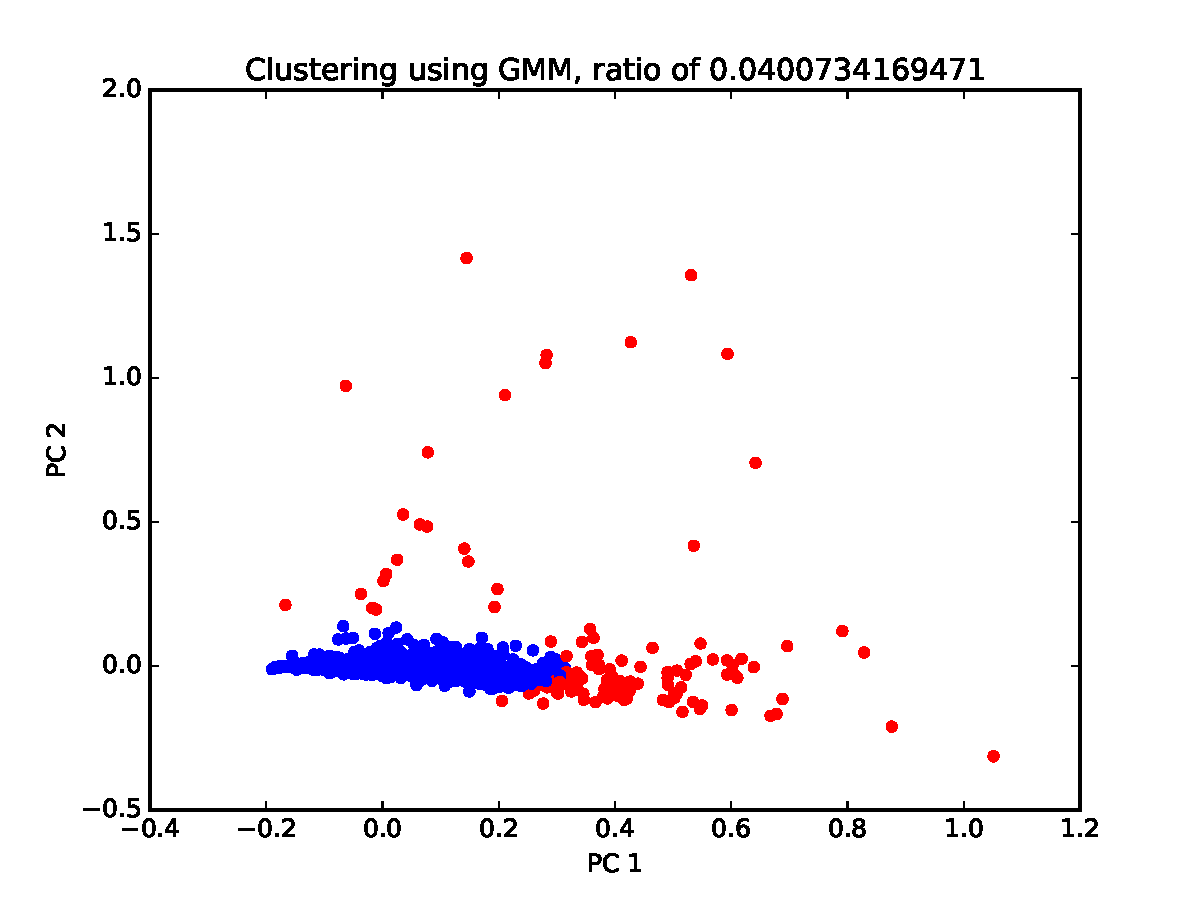
\includegraphics[width=.32\textwidth]{./img/comp_GMM_04.pdf}}
	\subfloat[Kmeans (19 \%)]{
		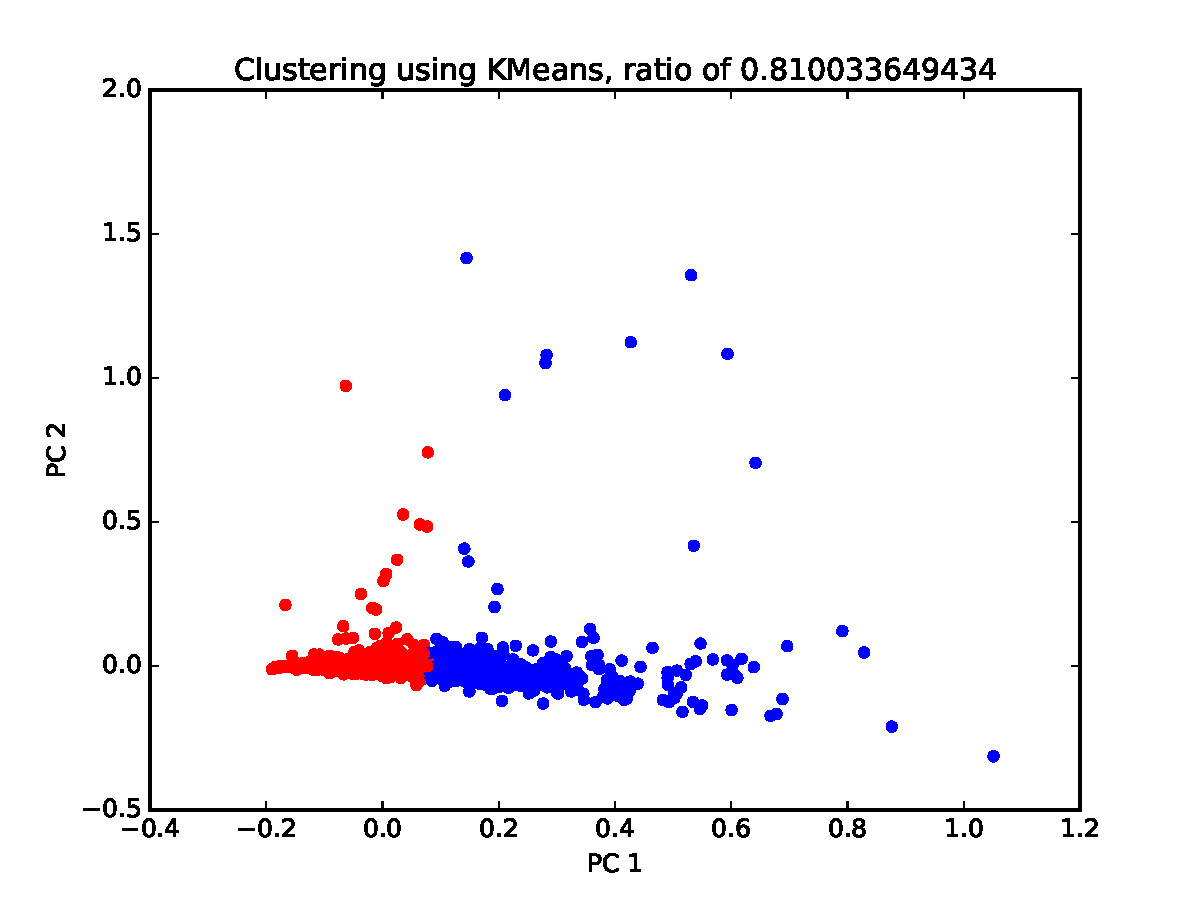
\includegraphics[width=.32\textwidth]{./img/comp_Kmeans_19.pdf}}
	\subfloat[Spectral Clustering (21 \%)]{
		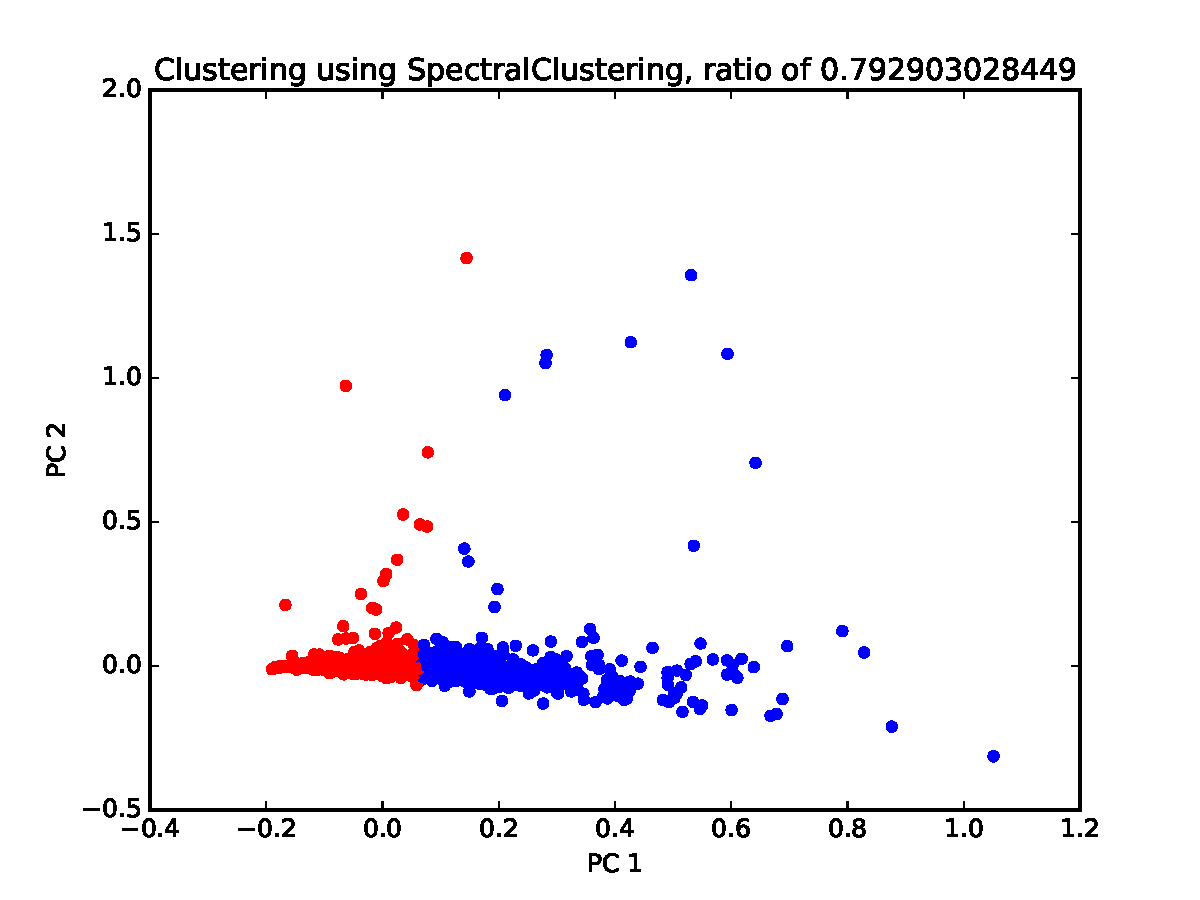
\includegraphics[width=.32\textwidth]{./img/comp_Spectral_21.pdf}}
		\caption{Clustering results when using different algorithms.}
	\label{fig_comparison}		
\end{figure}

\paragraph{Clustering Algorithm Choice Discussion}
I think there are two criteria when choosing the clustering algorithm. On the one hand, it is important that the result of the clustering does look similar to the results of the created benchmark. One the other hand, there is also a practical aspect that must be considered. To be usable by a tutor, the grouping must divide the students in groups that at least approximately of a similar size, as it is not very useful to design an aspect of an exercise that will probably affect less than one per cent of the students. Considering these criteria, the three algorithms that are chosen for further investigation are Agglomerative Clustering, Kmeans, and Spectral Clustering. As can be observed in Fig.~\ref{fig_comparison}, these three algorithms provide results which resemble the benchmark. At the same time, they all divide the data into two groups, where one of the groups is approximately 4 times the size of the other. Relatively to the problem at hand, these algorithms, when trained, will try to estimate whether a student is in the top 20 \% most able students. 

\subsubsection{Adjusting the Benchmark}
As outlined in the previous section, the chosen clustering algorithms divide the data into two groups, where one of the groups is approximately 4 times larger than the other one. Consequently, it appears sensible to adjust the benchmark that divides the students into to groups of equal size. The benchmark used hereafter is created by assigning the top 20 \% of the ordered correctness list to the first and the remaining 80 \% to the second group.


\subsubsection{Evaluating the Algorithms}
To compare the chosen algorithms, I evaluate them against the benchmark and measure the rate of true positives, true negatives, false positives, and false negatives. The measurement is done by the script \textbf{\emph{compare.py}}. The results of this measurement are illustrated in Tab.~\ref{tab_comparison}. The evaluations indicate that the three algorithms perform similarly well and provide an accuracy of about 70\%. Kmeans has a small disposition towards false positives, while Agglomerative Clustering rather classifies good students as bad. Spectral Clustering has nearly the same probability for false positives and for false negatives. As the performance of the three algorithms is very similar, I choose Kmeans as the algorithm for the clustering because it performs the clustering much faster than the other two.   


\begin{table}[b]
	\centering
	\caption{Performance comparison of the three algorithms considered for the clustering. The best value achieved in each category is highlighted with a bold font.\label{tab_comparison}}
	\begin{tabular}{llll}
		\toprule
		Performance Characteristic & Kmeans & Agglomerative & Spectral \\		
		\midrule
		True Positives & $4.894\%$ & $\boldsymbol{6.393\%}$ & $5.720\%$\\
		True Negatives & $\boldsymbol{66.41\%}$ & $64.03\%$ & $65.00\%$\\
		False Positives & $15.11\%$ & $\boldsymbol{13.61\%}$ & $14.29\%$\\
		False Negatives & $\boldsymbol{13.58\%}$ & $15.97\%$ & $14.99\%$\\
		Predicted as Good & $18.48\%$ & $22.36\%$ & $20.71\%$\\
		\bottomrule
	\end{tabular}
\end{table}

\subsubsection{Parameter Tuning}
In the last step I used the script \textbf{\emph{tune\_parameters.py}} to experiment with different parameter settings of the Kmeans algorithm. However, the changing the parameters had no significant effect on the performance in relation to the benchmark. Changing the number of Kmeans runs and the maximum number of iterations in each run did not have any effect at all, so that it can be assumed that the algorithms displays a solid convergence. Changing the initialization technique had a small and mixed effect, improving some of the performance characteristics while making other characteristics worse. All in all, tuning the parameters does not provide an improved result in comparison to the default settings. 

\subsubsection{Robustness Test}
To test the robustness of the created machine learning pipeline, I implemented a test, similar to those performed for the supervised classification. For this, I created a training and a test set consisting of the PC data of the students from the two principal components set. The training set is hereby created by randomly selecting 320 (roughly 10\% of the original set) student entries, while the training set contains all remaining entries. For convenience, I also create the test bench set, which contains the correction based classification for the 320 students selected for the test. The creation of these data sets is done using the script \textbf{\emph{create\_data\_set.py}}.

The robustness is then tested by training the KNN clusterer with the training data and then comparing the predictions the trained clusterer makes for the test data (that was not used during training) with the correction based classification of the test data. This is done by the script \textbf{\emph{test\_robustness.py}}. To evaluate the robustness, I use the same metrics as for the evaluation of the algorithm itself.

The results of the robustness test can be found in Tab.~\ref{tab_robustness}. The test values are very similar to the values obtained when using the full training set. The robustness test, hence, seems to indicate that the model created in this project is robust when confronted with unknown data and can be used as a part of the framework for exercise design (at least if the data set that this project is working with is representative for the students and problems from the computer science area).

\begin{table}[b]
	\centering
	\caption{Results of the robustness test.\label{tab_robustness}}
	\begin{tabular}{lll}
		\toprule
		Performance Characteristic & Absolute Value & Delta to Training Value \\		
		\midrule
		True Positives & $4.375\%$ & $-0.519\%$\\
		True Negatives & $68.12\%$ & $+1.71\%$\\
		False Positives & $14.38\%$ & $+0.8\%$\\
		False Negatives & $13.12\%$ & $-5.36\%$\\
		\bottomrule
	\end{tabular}
\end{table}

\subsection{Result Summary}
As a result of the data preprocessing and a comparison of different clustering algorithms, I have created a pipeline that fits a Kmeans algorithm to the provided student data. The fitted algorithm predicts whether a student's performance will be within the top 20\%. Compared with the presented benchmark, this predictor has an accuracy of 70\% and seems to be robust in the presence of unknown data. The relatively low accuracy probably results from the fact that the used benchmark is not a golden model, but instead classifies based on a single feature. As the created predictor takes many more features, in particular the time for the solution of a problem, into account, it is to be expected that its results differ from the chosen benchmark.

\subsection{Challenges during the Implementation}
During the implementation of the preprocessing and machine pipeline described in this section, I have encountered one difficulty.

%The first difficulty occurred during the creation of the student-centered data set. There, I have seen that, in the created set, some few students had nan entries for either the \emph{error step duration} of the \emph{correct step duration} feature. After some reflection, I have come to the conclusion that those were the students who either got all the problems right (in this case, the error step duration is a nan) or got all the problems wrong (then, the correct step duration is a nan). As the nan caused errors during the min-max scaling, I had to replace the nans in these cases by a value that \textbf{I} can be processed during min-max scaling and \textbf{II} can not be confused with one of the non-nan values. For these reasons, I decided to enter a -1 in these cases. 

The difficulty occurred during the calculation of the accuracy values that I used to measure the correlation between the clustering and a classification based on the average correctness. While the correctness function always assigned a 1 to the students in the upper part of the list, the clustering algorithms just separated the students into two groups. The labels for the individual groups, however, were not reproducible (sometimes, the 'better' students were assigned a 1 and at other times, they were assigned a 0). This made it difficult to automatically calculate the accuracy values. After making sure that the actual clustering always provides the same results regardless of the chosen labels and that it always predicts roughly 20\% students as gifted, I implemented a dynamic labeling, where the cluster with the bigger size (the less able students) was labeled with a 0, while the cluster with the smaller size (the gifted students) was labeled with a 1. This solved the problem.  


